% Options for packages loaded elsewhere
\PassOptionsToPackage{unicode}{hyperref}
\PassOptionsToPackage{hyphens}{url}
%
\documentclass[
  11pt,
  ignorenonframetext,
  handout]{beamer}
\usepackage{pgfpages}
\setbeamertemplate{caption}[numbered]
\setbeamertemplate{caption label separator}{: }
\setbeamercolor{caption name}{fg=normal text.fg}
\beamertemplatenavigationsymbolsempty
% Prevent slide breaks in the middle of a paragraph
\widowpenalties 1 10000
\raggedbottom
\setbeamertemplate{part page}{
  \centering
  \begin{beamercolorbox}[sep=16pt,center]{part title}
    \usebeamerfont{part title}\insertpart\par
  \end{beamercolorbox}
}
\setbeamertemplate{section page}{
  \centering
  \begin{beamercolorbox}[sep=12pt,center]{part title}
    \usebeamerfont{section title}\insertsection\par
  \end{beamercolorbox}
}
\setbeamertemplate{subsection page}{
  \centering
  \begin{beamercolorbox}[sep=8pt,center]{part title}
    \usebeamerfont{subsection title}\insertsubsection\par
  \end{beamercolorbox}
}
\AtBeginPart{
  \frame{\partpage}
}
\AtBeginSection{
  \ifbibliography
  \else
    \frame{\sectionpage}
  \fi
}
\AtBeginSubsection{
  \frame{\subsectionpage}
}
\usepackage{amsmath,amssymb}
\usepackage{lmodern}
\usepackage{iftex}
\ifPDFTeX
  \usepackage[T1]{fontenc}
  \usepackage[utf8]{inputenc}
  \usepackage{textcomp} % provide euro and other symbols
\else % if luatex or xetex
  \usepackage{unicode-math}
  \defaultfontfeatures{Scale=MatchLowercase}
  \defaultfontfeatures[\rmfamily]{Ligatures=TeX,Scale=1}
\fi
% Use upquote if available, for straight quotes in verbatim environments
\IfFileExists{upquote.sty}{\usepackage{upquote}}{}
\IfFileExists{microtype.sty}{% use microtype if available
  \usepackage[]{microtype}
  \UseMicrotypeSet[protrusion]{basicmath} % disable protrusion for tt fonts
}{}
\makeatletter
\@ifundefined{KOMAClassName}{% if non-KOMA class
  \IfFileExists{parskip.sty}{%
    \usepackage{parskip}
  }{% else
    \setlength{\parindent}{0pt}
    \setlength{\parskip}{6pt plus 2pt minus 1pt}}
}{% if KOMA class
  \KOMAoptions{parskip=half}}
\makeatother
\usepackage{xcolor}
\IfFileExists{xurl.sty}{\usepackage{xurl}}{} % add URL line breaks if available
\IfFileExists{bookmark.sty}{\usepackage{bookmark}}{\usepackage{hyperref}}
\hypersetup{
  pdftitle={R-programmering VT2022},
  pdfauthor={Johan Alenlöv},
  hidelinks,
  pdfcreator={LaTeX via pandoc}}
\urlstyle{same} % disable monospaced font for URLs
\newif\ifbibliography
\usepackage{color}
\usepackage{fancyvrb}
\newcommand{\VerbBar}{|}
\newcommand{\VERB}{\Verb[commandchars=\\\{\}]}
\DefineVerbatimEnvironment{Highlighting}{Verbatim}{commandchars=\\\{\}}
% Add ',fontsize=\small' for more characters per line
\usepackage{framed}
\definecolor{shadecolor}{RGB}{248,248,248}
\newenvironment{Shaded}{\begin{snugshade}}{\end{snugshade}}
\newcommand{\AlertTok}[1]{\textcolor[rgb]{0.94,0.16,0.16}{#1}}
\newcommand{\AnnotationTok}[1]{\textcolor[rgb]{0.56,0.35,0.01}{\textbf{\textit{#1}}}}
\newcommand{\AttributeTok}[1]{\textcolor[rgb]{0.77,0.63,0.00}{#1}}
\newcommand{\BaseNTok}[1]{\textcolor[rgb]{0.00,0.00,0.81}{#1}}
\newcommand{\BuiltInTok}[1]{#1}
\newcommand{\CharTok}[1]{\textcolor[rgb]{0.31,0.60,0.02}{#1}}
\newcommand{\CommentTok}[1]{\textcolor[rgb]{0.56,0.35,0.01}{\textit{#1}}}
\newcommand{\CommentVarTok}[1]{\textcolor[rgb]{0.56,0.35,0.01}{\textbf{\textit{#1}}}}
\newcommand{\ConstantTok}[1]{\textcolor[rgb]{0.00,0.00,0.00}{#1}}
\newcommand{\ControlFlowTok}[1]{\textcolor[rgb]{0.13,0.29,0.53}{\textbf{#1}}}
\newcommand{\DataTypeTok}[1]{\textcolor[rgb]{0.13,0.29,0.53}{#1}}
\newcommand{\DecValTok}[1]{\textcolor[rgb]{0.00,0.00,0.81}{#1}}
\newcommand{\DocumentationTok}[1]{\textcolor[rgb]{0.56,0.35,0.01}{\textbf{\textit{#1}}}}
\newcommand{\ErrorTok}[1]{\textcolor[rgb]{0.64,0.00,0.00}{\textbf{#1}}}
\newcommand{\ExtensionTok}[1]{#1}
\newcommand{\FloatTok}[1]{\textcolor[rgb]{0.00,0.00,0.81}{#1}}
\newcommand{\FunctionTok}[1]{\textcolor[rgb]{0.00,0.00,0.00}{#1}}
\newcommand{\ImportTok}[1]{#1}
\newcommand{\InformationTok}[1]{\textcolor[rgb]{0.56,0.35,0.01}{\textbf{\textit{#1}}}}
\newcommand{\KeywordTok}[1]{\textcolor[rgb]{0.13,0.29,0.53}{\textbf{#1}}}
\newcommand{\NormalTok}[1]{#1}
\newcommand{\OperatorTok}[1]{\textcolor[rgb]{0.81,0.36,0.00}{\textbf{#1}}}
\newcommand{\OtherTok}[1]{\textcolor[rgb]{0.56,0.35,0.01}{#1}}
\newcommand{\PreprocessorTok}[1]{\textcolor[rgb]{0.56,0.35,0.01}{\textit{#1}}}
\newcommand{\RegionMarkerTok}[1]{#1}
\newcommand{\SpecialCharTok}[1]{\textcolor[rgb]{0.00,0.00,0.00}{#1}}
\newcommand{\SpecialStringTok}[1]{\textcolor[rgb]{0.31,0.60,0.02}{#1}}
\newcommand{\StringTok}[1]{\textcolor[rgb]{0.31,0.60,0.02}{#1}}
\newcommand{\VariableTok}[1]{\textcolor[rgb]{0.00,0.00,0.00}{#1}}
\newcommand{\VerbatimStringTok}[1]{\textcolor[rgb]{0.31,0.60,0.02}{#1}}
\newcommand{\WarningTok}[1]{\textcolor[rgb]{0.56,0.35,0.01}{\textbf{\textit{#1}}}}
\usepackage{longtable,booktabs,array}
\usepackage{calc} % for calculating minipage widths
\usepackage{caption}
% Make caption package work with longtable
\makeatletter
\def\fnum@table{\tablename~\thetable}
\makeatother
\usepackage{graphicx}
\makeatletter
\def\maxwidth{\ifdim\Gin@nat@width>\linewidth\linewidth\else\Gin@nat@width\fi}
\def\maxheight{\ifdim\Gin@nat@height>\textheight\textheight\else\Gin@nat@height\fi}
\makeatother
% Scale images if necessary, so that they will not overflow the page
% margins by default, and it is still possible to overwrite the defaults
% using explicit options in \includegraphics[width, height, ...]{}
\setkeys{Gin}{width=\maxwidth,height=\maxheight,keepaspectratio}
% Set default figure placement to htbp
\makeatletter
\def\fps@figure{htbp}
\makeatother
\setlength{\emergencystretch}{3em} % prevent overfull lines
\providecommand{\tightlist}{%
  \setlength{\itemsep}{0pt}\setlength{\parskip}{0pt}}
\setcounter{secnumdepth}{-\maxdimen} % remove section numbering
\usetheme[progressbar=frametitle,block=fill]{metropolis} %numbering=none

%%% USEFUL PACKAGES
%\usepackage{showframe} % For debugging positioning
\usepackage{etex} % If too many packages
% Encoding and language
\usepackage[utf8]{inputenc}
\usepackage{babel}
\usepackage{amsmath, amssymb}
\usepackage{natbib}
%\usepackage{booktabs}
%\usepackage{algorithmic}
\usepackage{algorithm}
\usepackage{caption}
%\usepackage{animate} % Animations
\usepackage{bm} % Bold math
\usepackage{bbm}
%\usepackage{url}
%\usepackage{pifont}
%\usepackage{ulem} % Used for strikeouts \sout
%\usepackage{stackengine}
%\usepackage{enumitem}
%\setlist[description]{leftmargin=\parindent,labelindent=\parindent}
%\usepackage{colortbl} % Used for colored rows in tables


%%% GRAPHICS
\usepackage{graphicx}
\graphicspath{{./figs/}}


%%% COLORS
\setbeamercolor{background canvas}{bg=white}
\def\BlankFrame{
	\bgroup
	%\pdfpageheight 29.7cm
	\setbeamercolor{background canvas}{bg=}
	\begin{frame}[plain]
	\end{frame}
	%\makeatletter
	%\pdfpageheight \beamer@paperheight
	%\makeatother
	\egroup}

\usepackage{xcolor}
\definecolor{DarkGreen}{HTML}{00B200}
\definecolor{LightBlue}{HTML}{0090D9}
\definecolor{gold}{rgb}{.812,.710,.231}
% Text markup
%\setbeamercolor{alerted text}{fg=red}
\newcommand{\blue}[1]{\textcolor{blue}{#1}}
\newcommand{\red}[1]{\textcolor{red}{#1}}
\newcommand{\grey}[1]{\textcolor{gray}{#1}}
\newcommand{\orange}[1]{\textcolor{mLightBrown}{#1}}
\newcommand\myheading[1]{\textbf{#1}}
\newcommand\myemph[1]{\underline{\emph{#1}}}
\newcommand\textexample[1]{\textit{\textbf{#1}}}

%%% SPACING
\newcommand\vws[1][1]{\vspace{#1\baselineskip}} % vertical white space
%\newcommand\strt[1][1.5ex]{\rule[-.05\baselineskip]{0pt}{#1}} % strut
\newcommand\strt[2]{\rule[-#1ex]{0pt}{#2ex}} % strut
\newcommand\Hrule{\vspace{1ex} \hrule \vspace{1ex}} % Horisontal rule with some space after

%%% MISC
\newcommand\articleref[4]{\noindent\begin{minipage}[t]{0.04\textwidth}
		\vspace{0pt} 
		\pgfuseimage{beamericonarticle}
	\end{minipage}%
	\begin{minipage}[t]{0.96\textwidth}
		\vspace{0pt}
		#1. \textbf{#2.} \textit{#3}, #4.
	\end{minipage}}

%%% METROPOLIS THEME SPECIFIC
\makeatletter
\setlength{\metropolis@progressonsectionpage@linewidth}{1pt}
\makeatother
%\setbeamercolor{progress bar}{fg=red,bg=red!50}


%%% TEXTPOS
\usepackage[absolute,overlay]{textpos} % option showboxes is useful in draft mode
\setlength{\TPHorizModule}{\paperwidth}
\setlength{\TPVertModule}{\paperheight}
\textblockorigin{0pt}{10mm} % start everything at top-left, below gray 


%%% TIKZ/PGFPLOTS
\usepackage{tikz}
\usetikzlibrary{arrows,positioning,calc,shapes.geometric}
%\usetikzlibrary{arrows,calc,shapes.geometric,decorations.pathmorphing,backgrounds,positioning,fit,petri,decorations.pathreplacing}
%\usepackage{pgfplots}
%\pgfplotsset{compat = 1.3}


%%% BLOCKS AND BOXES
% Changing colors of blocks
%\setbeamercolor{block title alerted}{bg=UURed,fg=palette primary.fg}
%\setbeamercolor{block body alerted}{bg=UURed!15}
\setbeamercolor{block title alerted}{bg=mLightBrown,fg=palette primary.fg}
\setbeamercolor{block body alerted}{bg=mLightBrown!15}
%\setbeamercolor{block title example}{bg=UUGreen,fg=palette primary.fg}
%\setbeamercolor{block body example}{bg=UUGreen!10}
% \mybox is a rectangular box
\usepackage{boxedminipage}
\setlength\fboxrule{2pt}
\setlength\fboxsep{2\fboxsep}
\newcommand\mybox[3][\textwidth]{
  {\color{#2}
    \begin{boxedminipage}{#1}
      {\color{palette primary.bg} #3}
    \end{boxedminipage}}%
}   
\usepackage{tcolorbox}
\tcbset{arc=1mm,grow to left by=3mm,grow to right by=3mm,left=2mm}
%\newenvironment{redbox}{%
%	\begin{tcolorbox}[colback=UURed!15,colframe=UURed]}{%
%	\end{tcolorbox}}
%\newenvironment{greenbox}{%
%	\begin{tcolorbox}[colback=UUGreen!15,colframe=UUGreen]}{%
%	\end{tcolorbox}}
\newenvironment{redbox}{%
	\begin{tcolorbox}[colback=red!15,colframe=red]}{%
	\end{tcolorbox}}
\newenvironment{greenbox}{%
	\begin{tcolorbox}[colback=DarkGreen!15,colframe=DarkGreen]}{%
	\end{tcolorbox}}
\newenvironment{graybox}{%
	\begin{tcolorbox}[colback=mDarkTeal!5,colframe=mDarkTeal]}{%
	\end{tcolorbox}}
\newenvironment{orangebox}{%
\begin{tcolorbox}[colback=mLightBrown!15,colframe=mLightBrown]}{%
	\end{tcolorbox}}
\newenvironment{bwbox}{%
	\begin{tcolorbox}[colback=white,colframe=black]}{%
\end{tcolorbox}}
\newenvironment{bluebox}{%
	\begin{tcolorbox}[colback=LightBlue!15,colframe=LightBlue]}{%
\end{tcolorbox}}


%%%%%%%%% NEW MACROS

\newcommand\imp[1]{\alert{\textbf{#1}}}
\newcommand\bfit[1]{\textbf{\textit{#1}}}
\newcommand\good{\color{DarkGreen}{$\blacktriangle$}} % used in lists
\newcommand\bad{\color{red}{$\blacktriangledown$}} % used in lists

\ifLuaTeX
  \usepackage{selnolig}  % disable illegal ligatures
\fi

\title{R-programmering VT2022}
\subtitle{Föreläsning 7}
\author{Johan Alenlöv}
\date{2022-03-07}
\institute{Linköpings Universitet}

\begin{document}
\frame{\titlepage}

\hypertarget{fuxf6reluxe4sning-7}{%
\section{Föreläsning 7}\label{fuxf6reluxe4sning-7}}

\begin{frame}{Innehåll föreläsning 7}
\protect\hypertarget{innehuxe5ll-fuxf6reluxe4sning-7}{}
\begin{itemize}
\tightlist
\item
  Grafik med \texttt{ggplot2}
\item
  Grundläggande statistik
\item
  Linjär regression
\end{itemize}
\end{frame}

\hypertarget{ggplot2}{%
\section{ggplot2}\label{ggplot2}}

\begin{frame}{ggplot2}
\protect\hypertarget{ggplot2-1}{}
\begin{itemize}
\tightlist
\item
  Skapat av Hadley Wickham för över 10 år sedan
\item
  Baseras på ``Grammar of Graphics'' av Leland Wilkinson
\item
  Alternativ till basgrafiken
\item
  Grunden är alltid en \texttt{data.frame}
\end{itemize}
\end{frame}

\begin{frame}{Grammar of Graphics}
\protect\hypertarget{grammar-of-graphics}{}
\begin{itemize}
\tightlist
\item
  Abstraktion av grafiska idéer

  \begin{itemize}
  \tightlist
  \item
    Tänk språk med ordklasser/satsdeelar
  \end{itemize}
\item
  Ger ett teoretiskt ramverk för att bygga grafik.
\item
  Bygga upp grafik lager för lager
\end{itemize}
\end{frame}

\begin{frame}{ggplot2}
\protect\hypertarget{ggplot2-2}{}
\begin{itemize}
\tightlist
\item
  Bygger upp en graf av flera delar:

  \begin{itemize}
  \tightlist
  \item
    \texttt{data}: en \texttt{data.frame} med \textbf{all} data
  \item
    \texttt{aes}: asethetic mappings
  \item
    \texttt{geom}: geometriska objekt
  \item
    \texttt{facets}: subplottar
  \item
    \texttt{scales}: skalor
  \item
    \texttt{coordinate system}: koordinatsystem
  \end{itemize}
\end{itemize}
\end{frame}

\begin{frame}{ggplot2}
\protect\hypertarget{ggplot2-3}{}
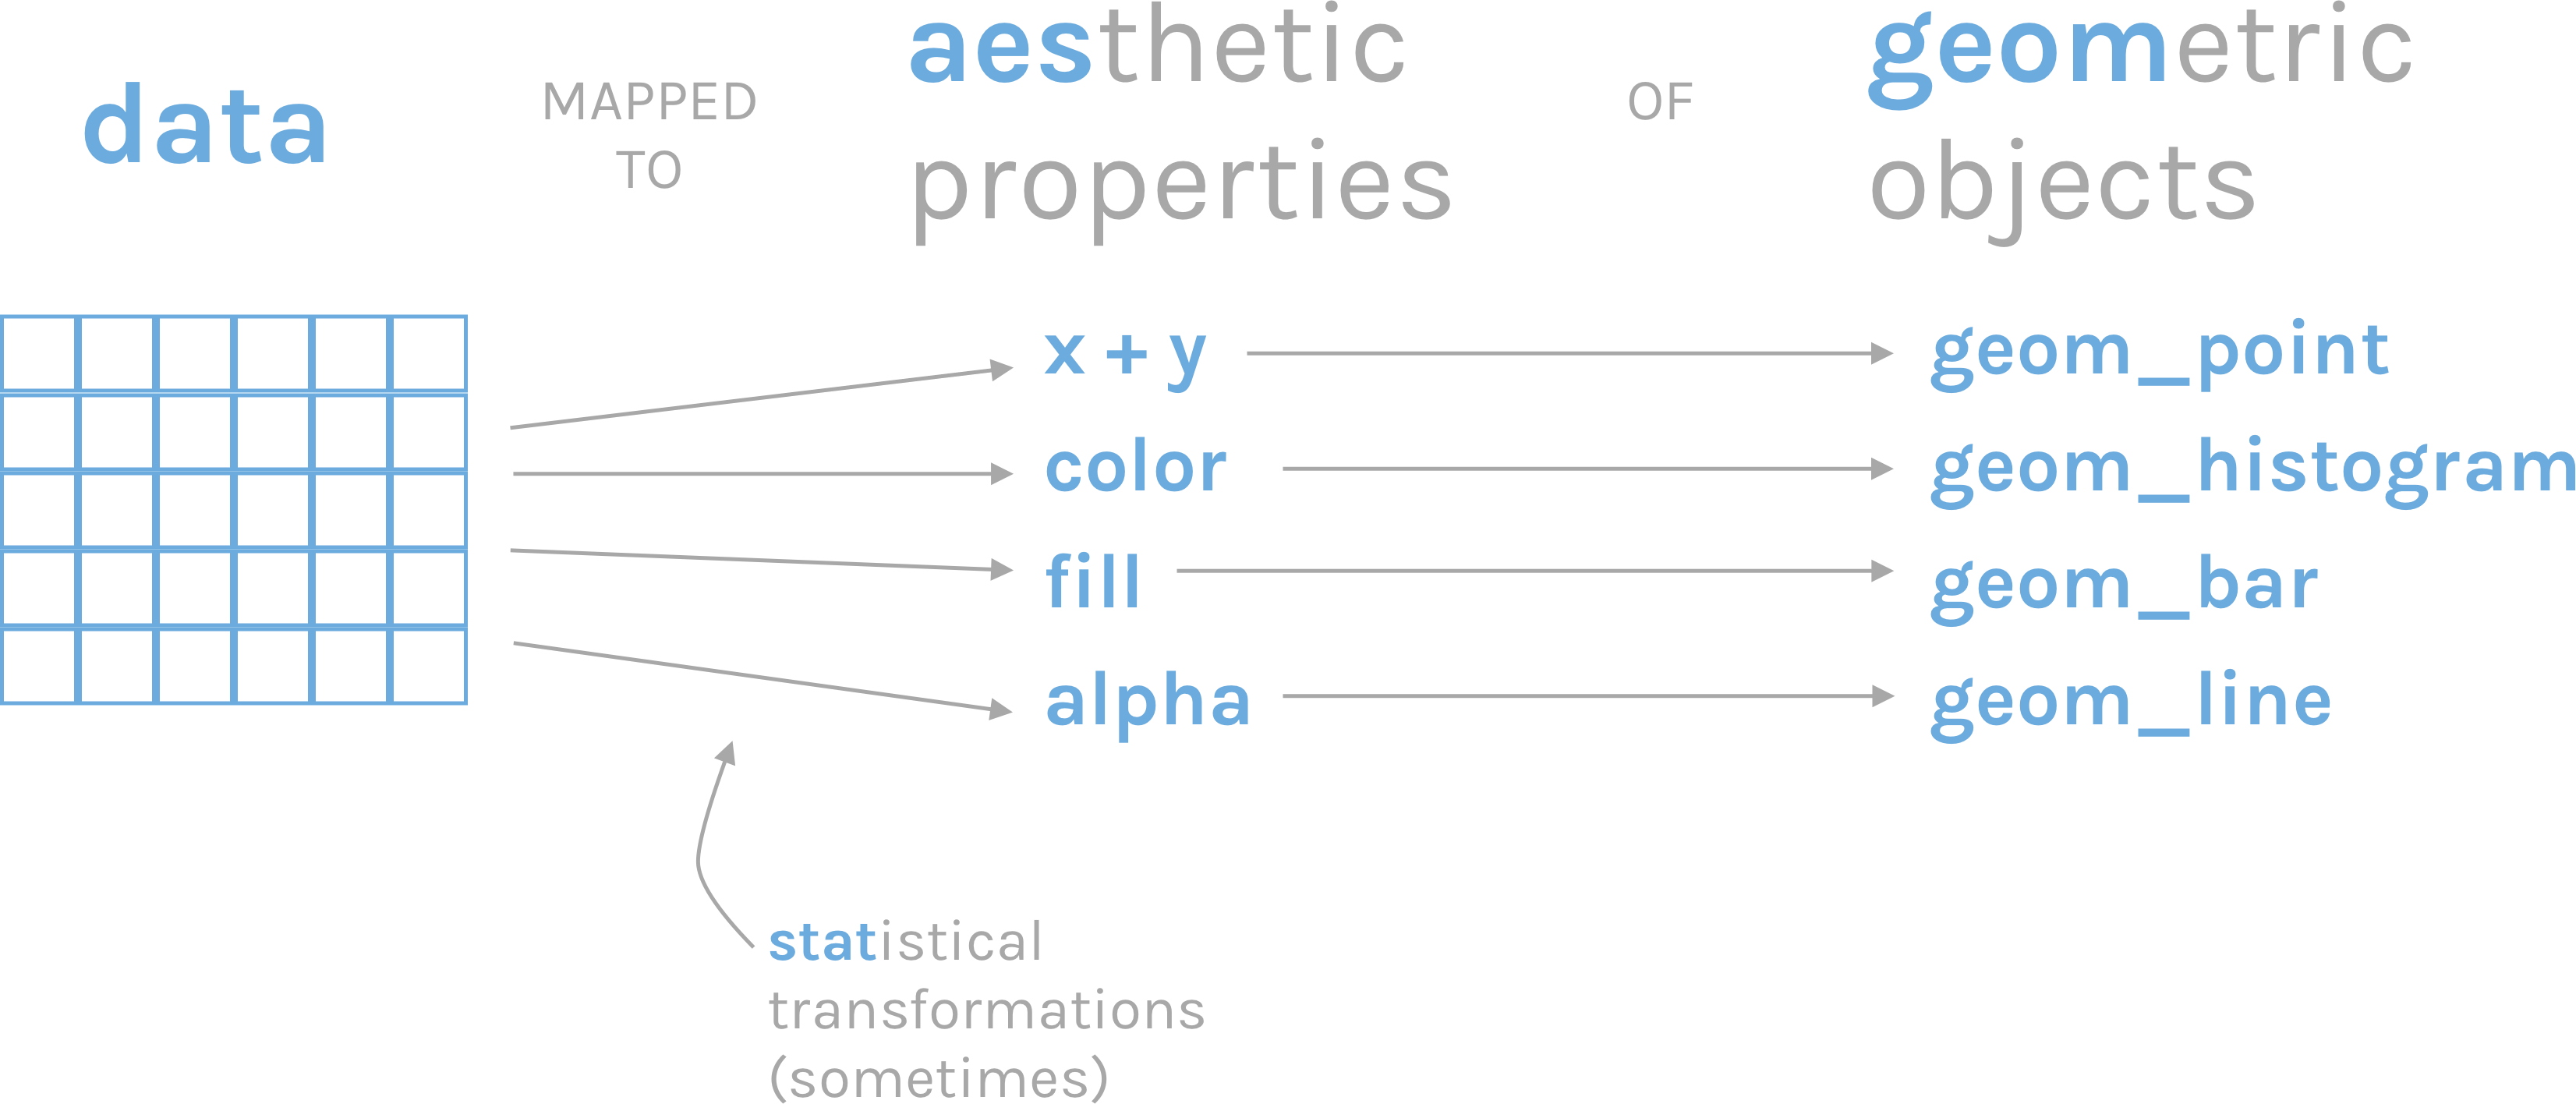
\includegraphics{images/grammar-of-graphics.png} Bild från ``R for the
rest of us''
\end{frame}

\begin{frame}{ggplot2}
\protect\hypertarget{ggplot2-4}{}
\begin{itemize}
\tightlist
\item
  \texttt{ggplot2} bygger upp en plot med olika lager

  \begin{itemize}
  \tightlist
  \item
    När plotten är klar så visas den
  \item
    Kan också visa med \texttt{print()}
  \end{itemize}
\item
  Utgår från \texttt{ggplot()}

  \begin{itemize}
  \tightlist
  \item
    Returnerar ett objekt
  \end{itemize}
\item
  Adderar lager med \texttt{+}

  \begin{itemize}
  \tightlist
  \item
    t.ex. \texttt{+ geom\_point()}
  \end{itemize}
\item
  Speciella klasser för \texttt{ggplot2}
\end{itemize}
\end{frame}

\begin{frame}{Grammar of Graphics}
\protect\hypertarget{grammar-of-graphics-1}{}
\begin{quote}
''In brief, the grammar tells us that a statistical graphic is a mapping
from data to aesthetic attributes (colour, shape, size) of geometric
objects (points, lines, bars). The plot may also contain statistical
transformations of the data and is drawn on a specific coordinate
system.''
\end{quote}

\emph{Från ``ggplot2 book'' av Hadley Wickham}
\end{frame}

\begin{frame}[fragile]{\textbf{aes}thetic (aes)}
\protect\hypertarget{aesthetic-aes}{}
Kopplar ihop färg, form och utseende till data

\begin{longtable}[]{@{}ll@{}}
\toprule
\texttt{aes} & Beskrivning \\
\midrule
\endhead
\texttt{x} & x-axel \\
\texttt{y} & y-axel \\
\texttt{size} & storlek \\
\texttt{color} & färg \\
\texttt{shape} & form \\
\bottomrule
\end{longtable}
\end{frame}

\begin{frame}[fragile]{geometric (geom)}
\protect\hypertarget{geometric-geom}{}
Vilken geometrisk representation ska användas

\begin{longtable}[]{@{}ll@{}}
\toprule
\texttt{geom} & Beskrivning \\
\midrule
\endhead
\texttt{geom\_point} & Scatterplot \\
\texttt{geom\_line} & Line graph \\
\texttt{geom\_bar} & Barplot \\
\texttt{geom\_boxplot} & Boxplot \\
\texttt{geom\_histogram} & Histogram \\
\bottomrule
\end{longtable}
\end{frame}

\begin{frame}[fragile]{aes och geom}
\protect\hypertarget{aes-och-geom}{}
Finns även speciella aesthetics för vissa geoms

\begin{longtable}[]{@{}ll@{}}
\toprule
\texttt{geom} & \texttt{aes} \\
\midrule
\endhead
\texttt{geom\_points} & point shape, point size \\
\texttt{geom\_line} & line type, line size \\
\texttt{geom\_bar} & y min, y max, fill color, outline color \\
\bottomrule
\end{longtable}
\end{frame}

\begin{frame}[fragile]{Exempel - I}
\protect\hypertarget{exempel---i}{}
\begin{Shaded}
\begin{Highlighting}[]
\FunctionTok{ggplot}\NormalTok{(}\AttributeTok{data =}\NormalTok{ Nile) }\SpecialCharTok{+} 
  \FunctionTok{aes}\NormalTok{(}\AttributeTok{x =}\NormalTok{ years, }\AttributeTok{y =}\NormalTok{ level) }\SpecialCharTok{+} 
  \FunctionTok{geom\_point}\NormalTok{()}
\end{Highlighting}
\end{Shaded}

\includegraphics{F7_johan_files/figure-beamer/unnamed-chunk-2-1.pdf}
\end{frame}

\begin{frame}[fragile]{Exempel - II}
\protect\hypertarget{exempel---ii}{}
\begin{Shaded}
\begin{Highlighting}[]
\FunctionTok{ggplot}\NormalTok{(}\AttributeTok{data =}\NormalTok{ Nile) }\SpecialCharTok{+} 
  \FunctionTok{aes}\NormalTok{(}\AttributeTok{x =}\NormalTok{ years, }\AttributeTok{y =}\NormalTok{ level) }\SpecialCharTok{+} 
  \FunctionTok{geom\_line}\NormalTok{()}
\end{Highlighting}
\end{Shaded}

\includegraphics{F7_johan_files/figure-beamer/unnamed-chunk-3-1.pdf}
\end{frame}

\begin{frame}[fragile]{Exempel - III}
\protect\hypertarget{exempel---iii}{}
\begin{Shaded}
\begin{Highlighting}[]
\FunctionTok{ggplot}\NormalTok{(}\AttributeTok{data =}\NormalTok{ Nile) }\SpecialCharTok{+} 
  \FunctionTok{aes}\NormalTok{(}\AttributeTok{x =}\NormalTok{ years, }\AttributeTok{y =}\NormalTok{ level, }\AttributeTok{color =}\NormalTok{ period) }\SpecialCharTok{+} 
  \FunctionTok{geom\_point}\NormalTok{(}\FunctionTok{aes}\NormalTok{(}\AttributeTok{shape =}\NormalTok{ period))}
\end{Highlighting}
\end{Shaded}

\includegraphics{F7_johan_files/figure-beamer/unnamed-chunk-4-1.pdf}
\end{frame}

\begin{frame}[fragile]{Exempel - IV}
\protect\hypertarget{exempel---iv}{}
\begin{Shaded}
\begin{Highlighting}[]
\FunctionTok{ggplot}\NormalTok{(}\AttributeTok{data =}\NormalTok{ Nile) }\SpecialCharTok{+} 
  \FunctionTok{aes}\NormalTok{(}\AttributeTok{x =}\NormalTok{ years, }\AttributeTok{y =}\NormalTok{ level, }\AttributeTok{color =}\NormalTok{ period) }\SpecialCharTok{+} 
  \FunctionTok{geom\_line}\NormalTok{() }\SpecialCharTok{+}
  \FunctionTok{geom\_point}\NormalTok{()}
\end{Highlighting}
\end{Shaded}

\includegraphics{F7_johan_files/figure-beamer/unnamed-chunk-5-1.pdf}
\end{frame}

\begin{frame}[fragile]{Exempel - V}
\protect\hypertarget{exempel---v}{}
\begin{Shaded}
\begin{Highlighting}[]
\FunctionTok{ggplot}\NormalTok{(}\AttributeTok{data =}\NormalTok{ Nile) }\SpecialCharTok{+} 
  \FunctionTok{aes}\NormalTok{(}\AttributeTok{x =}\NormalTok{ years, }\AttributeTok{y =}\NormalTok{ level) }\SpecialCharTok{+} 
  \FunctionTok{facet\_grid}\NormalTok{(period }\SpecialCharTok{\textasciitilde{}}\NormalTok{ .) }\SpecialCharTok{+} 
  \FunctionTok{geom\_line}\NormalTok{()}
\end{Highlighting}
\end{Shaded}

\includegraphics{F7_johan_files/figure-beamer/unnamed-chunk-6-1.pdf}
\end{frame}

\begin{frame}[fragile]{Exempel - VI}
\protect\hypertarget{exempel---vi}{}
\begin{Shaded}
\begin{Highlighting}[]
\NormalTok{p }\OtherTok{\textless{}{-}} \FunctionTok{ggplot}\NormalTok{(}\AttributeTok{data =}\NormalTok{ Nile) }\SpecialCharTok{+} 
  \FunctionTok{aes}\NormalTok{(}\AttributeTok{x =}\NormalTok{ years, }\AttributeTok{y =}\NormalTok{ level) }\SpecialCharTok{+} 
  \FunctionTok{facet\_grid}\NormalTok{(}\SpecialCharTok{\textasciitilde{}}\NormalTok{ period) }\SpecialCharTok{+} 
  \FunctionTok{geom\_line}\NormalTok{()}
\FunctionTok{print}\NormalTok{(p)}
\end{Highlighting}
\end{Shaded}

\includegraphics{F7_johan_files/figure-beamer/unnamed-chunk-7-1.pdf}
\end{frame}

\begin{frame}[fragile]{Exempel - VII : Teman}
\protect\hypertarget{exempel---vii-teman}{}
\begin{Shaded}
\begin{Highlighting}[]
\NormalTok{p }\SpecialCharTok{+} \FunctionTok{theme\_bw}\NormalTok{()}
\end{Highlighting}
\end{Shaded}

\includegraphics{F7_johan_files/figure-beamer/unnamed-chunk-8-1.pdf}
\end{frame}

\begin{frame}[fragile]{Exempel - VIII : Teman}
\protect\hypertarget{exempel---viii-teman}{}
\begin{Shaded}
\begin{Highlighting}[]
\NormalTok{p }\SpecialCharTok{+} \FunctionTok{theme\_calc}\NormalTok{()}
\end{Highlighting}
\end{Shaded}

\includegraphics{F7_johan_files/figure-beamer/unnamed-chunk-9-1.pdf}
\end{frame}

\begin{frame}[fragile]{Exempel - IX : Teman}
\protect\hypertarget{exempel---ix-teman}{}
\begin{Shaded}
\begin{Highlighting}[]
\NormalTok{p }\SpecialCharTok{+} \FunctionTok{theme\_clean}\NormalTok{()}
\end{Highlighting}
\end{Shaded}

\includegraphics{F7_johan_files/figure-beamer/unnamed-chunk-10-1.pdf}
\end{frame}

\begin{frame}[fragile]{Exempel - X : Teman}
\protect\hypertarget{exempel---x-teman}{}
\begin{Shaded}
\begin{Highlighting}[]
\NormalTok{p }\SpecialCharTok{+} \FunctionTok{theme\_minimal}\NormalTok{()}
\end{Highlighting}
\end{Shaded}

\includegraphics{F7_johan_files/figure-beamer/unnamed-chunk-11-1.pdf}
\end{frame}

\begin{frame}{\texttt{qplot}}
\protect\hypertarget{section}{}
\begin{itemize}
\tightlist
\item
  \texttt{qplot()} liknar \texttt{plot()}
\item
  Bra för snabba grafer
\item
  För mer kontroll använd \texttt{ggplot()}
\end{itemize}
\end{frame}

\hypertarget{statistik}{%
\section{Statistik}\label{statistik}}

\begin{frame}{Enklare statistika tester}
\protect\hypertarget{enklare-statistika-tester}{}
\begin{itemize}
\tightlist
\item
  Finns massor av olika statistiska tester

  \begin{itemize}
  \tightlist
  \item
    Väldigt många finns i R också
  \end{itemize}
\item
  För t-tester används \texttt{t.test()}
\item
  För \(\chi^2\)-tester används

  \begin{itemize}
  \tightlist
  \item
    \texttt{chisq.test()}, \texttt{fisher.test()}
  \end{itemize}
\item
  Korrelation och kovarians kan beräknas och testas

  \begin{itemize}
  \tightlist
  \item
    \texttt{cor()} och \texttt{cov()}
  \item
    \texttt{cor.test()}
  \end{itemize}
\end{itemize}
\end{frame}

\begin{frame}[fragile]{Exempel: t.test() - I}
\protect\hypertarget{exempel-t.test---i}{}
\begin{Shaded}
\begin{Highlighting}[]
\FunctionTok{data}\NormalTok{(}\StringTok{"chickwts"}\NormalTok{)}
\NormalTok{horsebean }\OtherTok{\textless{}{-}}\NormalTok{ chickwts}\SpecialCharTok{$}\NormalTok{weight[chickwts}\SpecialCharTok{$}\NormalTok{feed }\SpecialCharTok{==} \StringTok{"horsebean"}\NormalTok{]}
\NormalTok{sunflower }\OtherTok{\textless{}{-}}\NormalTok{ chickwts}\SpecialCharTok{$}\NormalTok{weight[chickwts}\SpecialCharTok{$}\NormalTok{feed }\SpecialCharTok{==} \StringTok{"sunflower"}\NormalTok{]}

\FunctionTok{mean}\NormalTok{(horsebean)}
\end{Highlighting}
\end{Shaded}

\begin{verbatim}
## [1] 160.2
\end{verbatim}

\begin{Shaded}
\begin{Highlighting}[]
\FunctionTok{mean}\NormalTok{(sunflower)}
\end{Highlighting}
\end{Shaded}

\begin{verbatim}
## [1] 328.9167
\end{verbatim}
\end{frame}

\begin{frame}[fragile]{Exempel: t.test() - II}
\protect\hypertarget{exempel-t.test---ii}{}
\begin{Shaded}
\begin{Highlighting}[]
\FunctionTok{t.test}\NormalTok{(horsebean, }\AttributeTok{alternative =} \StringTok{"two.sided"}\NormalTok{,}
       \AttributeTok{mu =} \DecValTok{150}\NormalTok{, }\AttributeTok{conf.level =} \FloatTok{0.95}\NormalTok{)}
\end{Highlighting}
\end{Shaded}

\begin{verbatim}
## 
##  One Sample t-test
## 
## data:  horsebean
## t = 0.83507, df = 9, p-value = 0.4253
## alternative hypothesis: true mean is not equal to 150
## 95 percent confidence interval:
##  132.5687 187.8313
## sample estimates:
## mean of x 
##     160.2
\end{verbatim}
\end{frame}

\begin{frame}[fragile]{Exempel: t.test() - III}
\protect\hypertarget{exempel-t.test---iii}{}
\begin{Shaded}
\begin{Highlighting}[]
\FunctionTok{t.test}\NormalTok{(horsebean, sunflower,}
       \AttributeTok{alternative =} \StringTok{"two.sided"}\NormalTok{,}
       \AttributeTok{mu =} \DecValTok{0}\NormalTok{, }\AttributeTok{conf.level =} \FloatTok{0.95}\NormalTok{)}
\end{Highlighting}
\end{Shaded}

\begin{verbatim}
## 
##  Welch Two Sample t-test
## 
## data:  horsebean and sunflower
## t = -9.0449, df = 19.964, p-value = 1.69e-08
## alternative hypothesis: true difference in means is not equal to 0
## 95 percent confidence interval:
##  -207.6313 -129.8021
## sample estimates:
## mean of x mean of y 
##  160.2000  328.9167
\end{verbatim}
\end{frame}

\hypertarget{linjuxe4r-regression}{%
\section{Linjär regression}\label{linjuxe4r-regression}}

\begin{frame}[fragile]{Linjär regression}
\protect\hypertarget{linjuxe4r-regression-1}{}
\begin{itemize}
\tightlist
\item
  I R finns formelobjektet som beskriver relationer mellan variabler

  \begin{itemize}
  \tightlist
  \item
    Formel skapas med \textasciitilde{}
  \item
    Exempel: \texttt{y\ \textasciitilde{}\ x1\ +\ x2}
  \end{itemize}
\item
  Att arbeta med modeller i R kan delas in i fyra steg:

  \begin{enumerate}
  \tightlist
  \item
    Anpassa (träna) en modell
  \item
    Analysera/studera resultatet
  \item
    Diagnostisera
  \item
    Använda modellen och resultaten
  \end{enumerate}
\item
  Linjär regression handlar om att hitta en linjär modell
\end{itemize}
\end{frame}

\begin{frame}[fragile]{Linjär regression - Anpassa en modell}
\protect\hypertarget{linjuxe4r-regression---anpassa-en-modell}{}
\begin{itemize}
\tightlist
\item
  Behöver en formel och data
\item
  Data behöver samma variabler som formeln
\end{itemize}

\begin{Shaded}
\begin{Highlighting}[]
\FunctionTok{library}\NormalTok{(MASS)}
\FunctionTok{library}\NormalTok{(car)}
\FunctionTok{data}\NormalTok{(Prestige)}
\end{Highlighting}
\end{Shaded}

\begin{Shaded}
\begin{Highlighting}[]
\NormalTok{mod1 }\OtherTok{\textless{}{-}} \FunctionTok{lm}\NormalTok{(prestige }\SpecialCharTok{\textasciitilde{}}\NormalTok{ income }\SpecialCharTok{+}\NormalTok{ women }\SpecialCharTok{+}\NormalTok{ education, }\AttributeTok{data=}\NormalTok{Prestige)}
\end{Highlighting}
\end{Shaded}

\begin{Shaded}
\begin{Highlighting}[]
\NormalTok{mod2 }\OtherTok{\textless{}{-}} \FunctionTok{lm}\NormalTok{(prestige }\SpecialCharTok{\textasciitilde{}}\NormalTok{ income }\SpecialCharTok{+}\NormalTok{ women }\SpecialCharTok{+}\NormalTok{ education }\SpecialCharTok{{-}} \DecValTok{1}\NormalTok{, }\AttributeTok{data=}\NormalTok{Prestige)}
\end{Highlighting}
\end{Shaded}

\begin{Shaded}
\begin{Highlighting}[]
\NormalTok{mod3 }\OtherTok{\textless{}{-}} \FunctionTok{lm}\NormalTok{(prestige }\SpecialCharTok{\textasciitilde{}}\NormalTok{ income}\SpecialCharTok{:}\NormalTok{women }\SpecialCharTok{+}\NormalTok{ education, }\AttributeTok{data=}\NormalTok{Prestige)}
\end{Highlighting}
\end{Shaded}
\end{frame}

\begin{frame}[fragile]{Linjär regression - Analysera modellen}
\protect\hypertarget{linjuxe4r-regression---analysera-modellen}{}
\begin{itemize}
\tightlist
\item
  Använd följande funktioner för att studera resultatet

  \begin{itemize}
  \tightlist
  \item
    \texttt{summary()}
  \item
    \texttt{anova()}
  \end{itemize}
\end{itemize}

Exempel:

\begin{Shaded}
\begin{Highlighting}[]
\FunctionTok{summary}\NormalTok{(mod1)}
\FunctionTok{anova}\NormalTok{(mod1)}
\FunctionTok{anova}\NormalTok{(mod1, mod2, }\AttributeTok{test =} \StringTok{"Chisq"}\NormalTok{)}
\end{Highlighting}
\end{Shaded}
\end{frame}

\begin{frame}[fragile]{Linjär regression - Diagnostisera}
\protect\hypertarget{linjuxe4r-regression---diagnostisera}{}
\begin{itemize}
\tightlist
\item
  Finns ett antal olika metoder, ex:
\end{itemize}

\begin{Shaded}
\begin{Highlighting}[]
\FunctionTok{plot}\NormalTok{(mod1)}
\FunctionTok{durbinWatsonTest}\NormalTok{(mod1)}
\FunctionTok{qqplot}\NormalTok{(mod1)}
\end{Highlighting}
\end{Shaded}
\end{frame}

\begin{frame}{Linjär regression - Använda modellen}
\protect\hypertarget{linjuxe4r-regression---anvuxe4nda-modellen}{}
\begin{itemize}
\tightlist
\item
  När vi har en modell kan vi göra olika saker:

  \begin{itemize}
  \tightlist
  \item
    Publicera modellen
  \item
    Studera residualer
  \item
    Prediktion
  \end{itemize}
\item
  Vi kan spara vår modell och använda

  \begin{itemize}
  \tightlist
  \item
    \texttt{resid()}
  \item
    \texttt{predict()}
  \end{itemize}
\end{itemize}
\end{frame}

\end{document}
